\documentclass[11pt,a4paper]{article}
\usepackage[a4paper, margin=1.3in]{geometry}
\usepackage{mathtools}
\usepackage{graphicx}
\usepackage{fancyhdr}
\pagestyle{fancy}
\fancyhf{}
\lhead{AI Planning}
\rhead{Exercise Sheet 3}
\lfoot{Axel Perschmann, Tarek Saier, 13.11.2014}
\rfoot{Page \thepage\ of 2}
\renewcommand{\headrulewidth}{0.3pt}
\renewcommand{\footrulewidth}{0.3pt}
\setlength\parindent{0pt}

\newcommand{\h}[0]{\text{--}}

\begin{document}
\begin{center}
\Huge{\textbf{AI Planning}}\\
\LARGE{\textbf{Exercise Sheet 3}}
\end{center}
\vspace{2cm}
\begin{tabular}{ll}
Date: & 13.11.2014\\
Students: & Axel Perschmann, Tarek Saier
\end{tabular}

\section*{Exercise 3.1}
See hand written notes.

\section*{Exercise 3.2}
(d=dancing, h=at-home, w=work, ro=romeo, ju=juliet)\\
We start at: $\gamma=ju\h d\land ro\h h$\\
We want to reach: $I=\{ro\h h\mapsto1,ju\h h\mapsto1\}$\\
Operators: $go\h d$, $go\h w$, $go\h h$\\
\\
$regr_{go\h w}(\gamma)=ro\h h\land$\\
\hphantom{aaaa}$((EPC_{ju\h d}(e_{go\h w})\lor (ju\h d\land \neg EPC_{\neg ju\h d}(e_{go\h w})))\land$\\
\hphantom{aaaaaa}$(EPC_{ro\h h}(e_{go\h w})\lor (ro\h h\land \neg EPC_{\neg ro\h h}(e_{go\h w})))$\\
\hphantom{aaaa}$) \land \kappa$\\
$regr_{go\h w}(\gamma)=ro\h h\land$\\
\hphantom{aaaa}$((\bot \lor (ju\h d\land \top))\land$\\
\hphantom{aaaaaa}$(\bot \lor (ro\h h\land \bot))$\\
\hphantom{aaaa}$) \land \kappa$\\
$regr_{go\h w}(\gamma)=\bot$\\
$\Rightarrow \gamma \text{ is not reachable by means of } go\h w$\\
\\
$regr_{go\h h}(\gamma)=ro\h w\land$\\
\hphantom{aaaa}$((\bot \lor (ju\h d\land \top))\land$\\
\hphantom{aaaaaa}$(EPC_{ro\h h}(e_{go\h h})\lor (ro\h h\land \neg EPC_{\neg ro\h h}(e_{go\h h})))$\\
\hphantom{aaaa}$) \land \kappa$\\
$regr_{go\h h}(\gamma)=ro\h w\land$\\
\hphantom{aaaa}$((\bot \lor (ju\h d\land \top))\land$\\
\hphantom{aaaaaa}$\top$\\
\hphantom{aaaa}$) \land \kappa$\\
$regr_{go\h h}(\gamma)=ro\h w\land ju\h d$\\
$\Rightarrow \gamma \text{ is reachable from }ro\h w\land ju\h d \text{ by means of } go\h h$\\
\\
//Note: less verbose from this point onwards.\\
\\
$regr_{go\h d}(\gamma)=ju\h h\land \top \land (\bot \lor (ro\h h \land \neg ro\h h)) \land \kappa= \bot$\\
$\Rightarrow \gamma \text{ is not reachable by means of } go\h d$\\
$\Rightarrow$ the only node to expand from is $n_1=ro\h w\land ju\h d$\\
\\
$regr_{go\h w}(n_1)=ro\h h\land ju\h d$ \hphantom{aaaa}(similar to $\gamma$, no further expansion)\\
$regr_{go\h h}(n_1)=\bot$\\
$regr_{go\h d}(n_1)=ro\h w\land ju\h h$ \hphantom{aaaa}($=n_2$)\\
\\
$regr_{go\h w}(n_2)=ro\h h\land ju\h h$ \hphantom{aaaa}($=n_3\models I$)\\
\\
\textbf{Resulting search tree:}\\
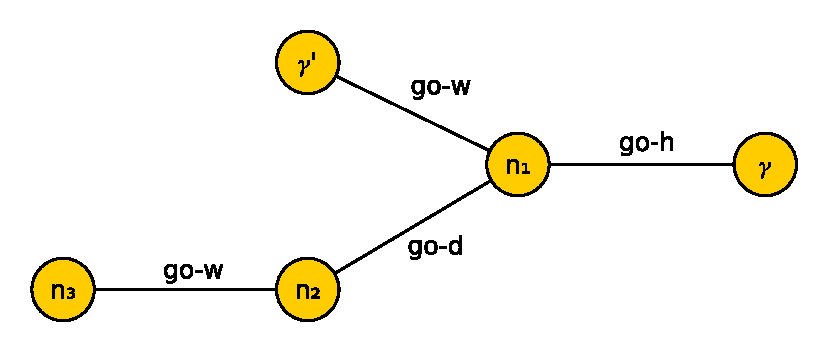
\includegraphics[scale=0.7]{search_tree}\\
\textbf{Resulting plan:}\\
$go\h w$, $go\h d$, $go\h h$
\end{document}
